\chapter{English-German}
\label{chap:german}

In this chapter we describe changes we have made to an existing
English-Czech MLFix pipeline to be able to apply the system to the English-German
SMT outputs. We summarize the data available for training the models
and evaluate the system in a similar way we did with the English-Czech
pipeline.

\section{Processing Pipeline Modifications}

As we have already pointed out, we have focused on making the processing pipeline as independent
on the target language as possible. However, we still have to replace some of the tools
used during the Czech analysis to be able to correctly process German sentences.

Again, we have used the Treex framework as a backbone of the processing pipeline and
necessary 3rd party tools were implemented into the systems via wrappers.
After the sentences are read in parrallel, they are processed separately, English
following the same scenario as in the English-Czech pipeline.
German is tokenized, this time by a set of regex rules inspired by Tiger corpus \citep{Brants2004}
with main focus on abbreviations, ordinal numbers and compounds connected by hyphens.

Next, lemmatization and POS tagging is performed by a Mate tools\footurl{http://www.ims.uni-stuttgart.de/forschung/ressourcen/werkzeuge/matetools.en.html}
toolkit. The tagger is using CoNLL2009 \citep{CoNLL-2009-ST} tagset. We have also considered using
Stanford POS Tagger \citep{Toutanova:2000:EKS:1117794.1117802}\footurl{http://nlp.stanford.edu/software/tagger.shtml},
however, the tagset it uses contains only coarse tags with little morphological information.
To convert the CoNLL2009 tags to Interset, we use a decoder which was already implemented at the
time of our research.

For the word alignment, we use GIZA++ again. Similar to English-Czech, we produce one-to-one word alignment
via intersetion symmetrization. The alignment model has been trained on the European
Parliament Parallel corpus \citep{koehn2005epc}\footnote{http://www.statmt.org/europarl/} (Europarl)
containing nearly two million sentences. During the process of training data analysis we 
also create monolingual alignment between the MT output and the references sentences
in a similar way we did in the original pipeline.

The dependency structure for the MT output is produced by projecting the English dependency
structures on the MT sentences. When we process the training data, we parse the reference sentences
by graph-based parser implementation \citep{Bohnet:2010:VHA:1873781.1873792} which is also a part of the
Mate tools toolkit. We stop the analysis at the a-layer, but again, in the future, further analyzing
the sentences to the t-layer to gain additional features for extraction might be helpful.

We have reused the statistical component used in the English-Czech pipeline, because it was designed to be
language independent (with the exception of the statistical models). For wordform generation we use
Flect morphology generation tool mentioned earlier. We have trained the generator on a small
fraction (around one hundred thousand sentences) of the Europarl corpus. The tool is trained on a set
of features based on a combination of lemma$+$Interset producing the inflected word. The feature set
was copied from the Dutch feature set so it might not contain all the useful features. The accuracy
of the inflection model measured on a separate test set was around 94.5\%. However, when we briefly examined
the sentences produced via Oracle, we have noticed that much larger amount of words was flected incorrectly.

It is not in the scope of this thesis but it is a future goal to replace the current inflection model
with a better solution, either stochastic or rule-based.

\section{Data Analysis}

We have been able to collect only a smaller variety of data for English-German compared to English-Czech,
 mostly due to some datasets we mentioned earlier were simply not available for this language pair. Still, we have been
able to gather following datasets: WMT16, HimL and Autodesk. Note that in case of Autodesk dataset,
the size of English-German is about three times bigger than the size of English-Czech (around 120k sentences).
For this reason, we have decided to include Autodesk dataset into our training data even though it covers
a quite specific domain.

When extracting the training instances for the model training we have followed same scenario
as before, using the same heuristic to identify \equo{incorrect} wordforms. We have also used the Oracle
classifier to gather information about possible improvements this heuristic can bring when applied to German.

We have also performed quick manual evaluation of the output produced by the Oracle classifier by a non-native
German speaker.
We have performed the evaluation on the WMT16 dataset this time because we have thought that medical domain of HimL dataset
would be too difficult for a non-native speaker to evaluate.
Due to limited
resources we have again used only a single annotator for this evaluation task. The evaluator, not being familiar
with the MLFix system, was presented set of instances containing the following: randomly shuffled MT output and Oracle output,
the source English sentence and the German reference translation. The results of the evaluation a shown in the~\Tref{oracle_de-maneval}.
We have decided to only correct morphological categories by Oracle leaving the surface form generation to Flect module because
we wanted to see the best possible outcome that can be achieved by the statistical fixing components. In the future
the Oracle evaluation with \equo{Oracle} surface form generation might also be a valuable source of information.
This choice likely resulted in worse performance of Oracle classifier when compared to Czech Oracle. Therefore
we still chose to use the same heuristic for marking incorrect instances in the training data.

\begin{table*}[t]
\centering
\small

\begin{tabular}{l|cc|ccc|cc}
Reference  &  Evaluated  &  Changed  &  $+$  &  $-$  &  0  &  Precision  &  Impact  \\
\hline
Post-edits  &  800  &  77  &  20  &  39  &  18  &  33.9\%  &  2.5\%  \\
\end{tabular}
\caption[Manual evaluation of the German Oracle classifier]{
Results of the the manual evaluation of the ideal fixing module based on the same heuristic
that was used in the English-Czech pipeline (WrongFrom3). Sentences were taken from HimL dataset. For wordform generation, a statistical component
was used impacting the overall performance.
}
\label{oracle_de-maneval}
\end{table*}

After the evaluation of the data extraction method we have analyzed the extracted instances and compared them
to the information we have gathered during Czech data analysis. \Fref{iset_de-barplot} shows the frequency of the changed Interset
categories. Again, case was the most changed category among our data followed by gender and number, either as a standalone change or
as a part of a clustered change. This led us to training the category prediction models in a same manner as in the English-Czech
pipeline with exception of the animateness (\pojem{CNGA}) models. To make sure that we can make similar assumptions during
the model development we have also checked distribution of changes per individual POS classes, The summary is shown in~\Tref{changes_de-pos}.
Even though the distribution is slightly different, nouns and adjectives are still teh most changed words which further supports
our decision for training Case, CN and CNG models.

\begin{figure}
\centering
  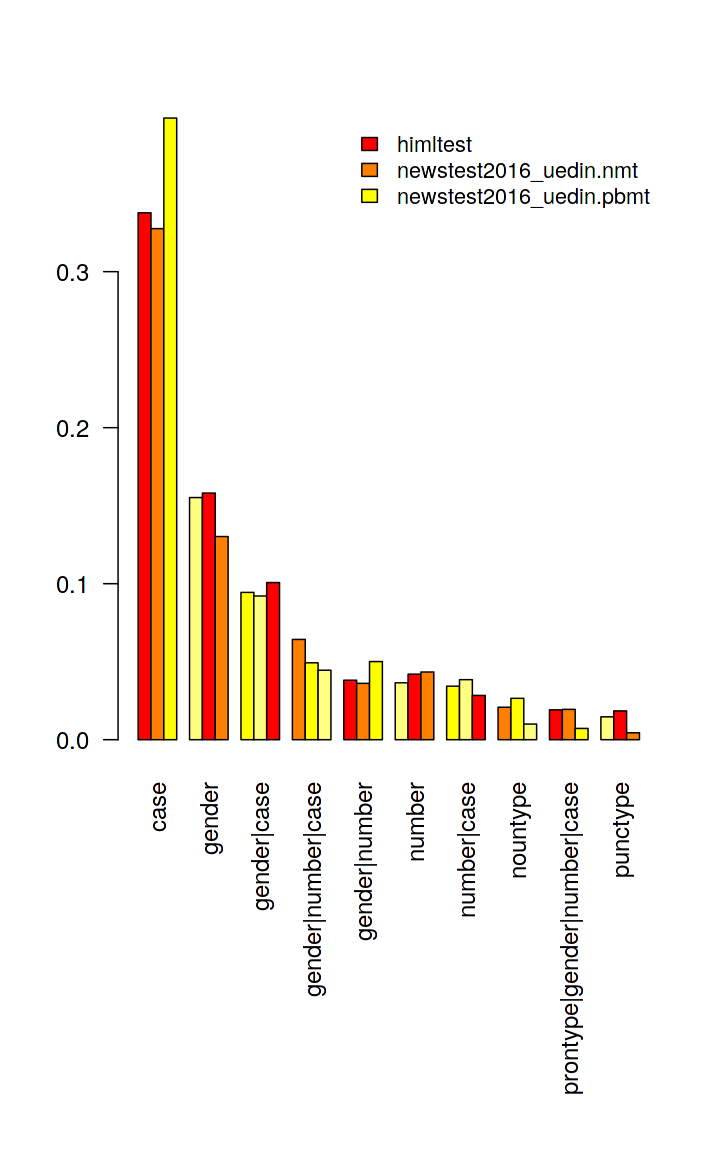
\includegraphics[scale=0.7]{iset_de}
  \caption[Change frequency of German morphological categories]{
    Frequency of the most changed Interset categories in German data, grouped by a datasets. Categories containing
    "\textbar" symbol (e.g. gender\textbar{}number) represent changes made simultaneously.
}
  \label{iset_de-barplot}
\end{figure}

\begin{table*}[t]
\centering
\small

\begin{tabular}{lc}
POS  &  Frequency  \\
\hline
noun    &   35\%  \\
adj     &   25\%  \\
punc	&	10\%  \\
adp     &   8\%  \\
conj    &   7\%  \\
\end{tabular}
\caption{
	Change frequency of various POS classes in German.
%    Part-of-speech (POS) frequencies of the changed words. Only the 5 most
%	frequent classes are displayed.
}
\label{changes_de-pos}
\end{table*}


\section{Model Developement}

We have skipped the process of choosing proper ML and feature selection method
assuming that the ones used for training models for English-Czech pipeline should
be also sufficient for German. We have only searched for the best combination
of hyperparameters during model development process. We have used both source
and MT features with addition of the source language lemmas. We present a summary
of the available training data for both error detection and morphological prediction in~\Tref{wf-cat-data-sum}.
Again, we can see, that the training data are quite small with exception of the Autodesk
dataset. That is also the main motivation behind including it in our training data.

\begin{table*}[t]
\centering
\small

\begin{tabular}{ll|ccc}
Dataset  &  System &  \hash{} Instances  &  \hash{} Instances (filt.)  &  \hash{} Incorrect  \\
\hline
HimL  &  Moses  & 12,067  &  2,729  &  369  \\
WMT16  &  UEDIN-NMT  &  22,353  &  3,340  &  344  \\
WMT16  &  UEDIN-PBMT  &  21,394  &   3,727  &  412  \\
Autodesk  &  $-$  &  1,263,750  &  124,698  &  17,268  \\
\end{tabular}
\caption[Summary of the extracted German training data]{
    Summary of the size of the training data extracted from each dataset. We present
size before and after (filt.) removing the instances extracted from the \equo{correct} sentences.
The size of datasets for category predictor training is presented in the \pojem{Incorrect} column.
}
\label{wf-cat-data-sum}
\end{table*}

The summary of the final error detection models is in~\Tref{wf_de-summary}. Surprisingly,
while having quite similar precision to the Czech models they achieved much better
recall overall. At this moment, we cannot say if it is caused by a ML method choice or a suitable
initial feature set, however, since there is still room for improvement, we consider investigating
the issue furter in the future.

\begin{table*}[t]
\centering
\small

\begin{tabular}{ll|ccc}
Dataset  &  System  &  Precision  &  Recall  &  F1  \\
\hline
HimL  &  Moses  &  0.39  &  0.56  &  0.46  \\
WMT16 &  UEDIN-NMT  &  0.28  &  0.43  &  0.34  \\
WMT16 &  UEDIN-NMT  &  0.29  &  0.50  &  0.37  \\
Autodesk  &  $-$  &  0.41  &  0.77  &  0.53  \\
\end{tabular}
\caption[Model summary (German) - error detection]{
    Summary of the in-domain performance of the final German error detection models.
}
\label{wf_de-summary}
\end{table*}

In~\Tref{cats_de-summary}, we present performance of the final German
mophology prediction models. The results are fairly similar to Czech models with
HimL model being slightly better, possibly due to a lesser amount of possible values
of the case category. Surprisingly, the accuracy of  a model trained on the Autodesk
dataset drops only a little with increasing complexity suggesting that increasing
the amount of training data can significantly improve the overall accuracy of the
resulting model.

\begin{table*}[t]
\centering
\small

\begin{tabular}{ll|ccc}
Dataset  &  System  &  Case(Base)  &  CN(Base)  & CNG(Base)  \\
\hline
HimL  &  Moses  &  84\%(29\%)  &  79\%(13\%)  &  70\%(5\%)  \\
WMT16  &  UEDIN-NMT  &  57\%(46\%)  &  48\%(27\%)  &  34\%(22\%)  \\
WMT16  &  UEDIN-PBMT  &  57\%(38\%)  &  47\%(21\%)  &  35\%(18\%)\\
Autodesk  &  $-$  &  96\%(28\%)  &  95\%(17\%)  &  93\%(8\%)  \\

\end{tabular}
\caption[Model summary (German) - morphological prediction]{
    Summary of the in-domain performance of the final German category prediction models
	and its comparison with the baseline predictor.
}
\label{cats_de-summary}
\end{table*}

\section{Evaluation}

We have followed same procedure during German MLFix evaluation as we followed during
Czech evaluation. We have compared several configurations of the morphological prediction
module and error detection module separately first, using Oracle to substitute the other
module, then we have evaluated the whole MLFix system. We have compared same configurations
we have used in Czech MLFix: \pojem{Case}, \pojem{CN}, \pojem{CNG} and \pojem{Combined} model configuration for morphology
prediction and \pojem{Majority}, \pojem{AtLeastOne} and \pojem{Average} voting scheme for error
detection. For the whole system evaluation, we have picked two most promising configurations
and compared their performance. We have also measured a performance of the best Czech configuration
(using Czech models) when applied to German. We have used BLEU score during automatic evaluation.
The evaluation was performed on the following datasets: Autodesk, HimL Lingea logs and WMT16.

We present the results of morphological prediction module evaluation in~\Tref{fixonly_de-summary}.
Once again, CNG configuration proved to be the reliable choice, having best score on each dataset.
However, the overall improvement in BLEU score is much lower when compared with Czech version
of MLFix. This is little surprising because the individual performance of the morphological prediction
models measured during training was equal and in some cases better than the one of the Czech models.
It is possible that this might be either a result of lower diversity in our data (most of the data belongs
to Autodesk dataset) or a consequence of the poor performance of the iflection module.

\begin{table*}[t]
\centering
\small
\resizebox{0.98\textwidth}{!}{

\begin{tabular}{|l|l||c||c||c|c|c|c|c|c|}
\hline
Dataset  &  System  &  Oracle  &  Base  &  Case  &  CN  & CNG  & Comb  \\
\hline
\hline
Autodesk  &  $-$  &  46.23  &  45.90  &  45.96 (+0.06)  &  45.95 (+0.05)  &  \bf{46.02} (+0.12)  &  45.98 (+0.08)  \\
\hline
HimL  &  Moses &  31.94  &  30.95  &  31.37 (+0.41)  &  31.29 (+0.34)  &  \bf{31.59} (+0.63)  &  31.46 (+0.50)\\
\hline
\multirow{2}{*}{WMT16}  &  UEDIN NMT  &  35.05  &  34.82  &  34.82 (0)  &  34.82 (0)  &  34.82 (0)  &  34.82 (0) \\
&  UEDIN PBMT  &  29.38  &  29.11  &  29.11 (0)  &  29.11 (0)  &  29.11 (0)  &  29.11 (0)  \\
\hline
\end{tabular}

}
\caption[Automatic evaluation of the German morphological prediction module]{
    Automatic evaluation of German morphological prediction module using BLEU metric
	and the relative improvement over the baseline MT output.
	Values are multiplied by 100 for easier reading.
	Performance of
	Oracle classifier is provided for comparison.
	The best model for each dataset is printed in bold.
}
\label{fixonly_de-summary}
\end{table*}


In~\Tref{markonly_de-summary}, we present the results of the evaluation of the error detection module.
We can see, that the module was performing quite poorly, not bringing any improvement to any dataset att all. Due to the nature of the error detection module evaluation (new morphological categories are taken from the reference sentences), we suspect that the main reason behind the poor performance is truly the
inflection module. Aside from that, we can see that this time it was the Majority scheme which performed
 much better than the rest. However, the results might only point to the fact that the Majority scheme
 marked the smallest number of instances as incorrect thus worsening the MT output much less than the
 other two.

\begin{table*}[t]
\centering
\small
\resizebox{0.98\textwidth}{!}{

\begin{tabular}{|l|l||c||c||c|c|c|c|c|c|}
\hline
Dataset  &  System  &  Oracle  &  Base  &  Majority  &  AtLeastOne  & Average  \\
\hline
\hline
Autodesk  &  $-$  &  46.23  &  45.90  &  \bf{45.80} (-0.10)  &  45.52 (-0.38)  &  45.79 (-0.11)  \\
\hline
HimL  &  Moses &  31.94  &  30.95  &  \bf{30.89} (-0.05)  &  30.17 (-0.77)  &  30.58 (-0.36)  \\
\hline
\multirow{2}{*}{WMT16}  &  UEDIN NMT  &  35.05  &  34.82  &  \bf{33.25} (-1.56)  &  30.15 (-4.67)  &  30.78 (-4.03)  \\
&  UEDIN PBMT  &  29.38  &  29.11  &  \bf{27.96} (-1.15)  &  25.41 (-3.7)  &  25.97 (-3.14)  \\
\hline
\end{tabular}

}
\caption[Automatic evaluation of the German error detection module]{
    Automatic evaluation of the error detection module using different voting methods to interpret output
of mutliple models using BLEU metric. Values are multiplied by 100 for easier reading,
and the relative improvement over the baseline MT output.
Performance of the
Oracle classifier is provided for comparison.
The best model for each dataset is printed in bold.
}
\label{markonly_de-summary}
\end{table*}

Nevertheless, we have decided to pick \pojem{Majority-CNG} and \pojem{Average-CNG} configurations
for the final evaluation. Their performance is summarized in~\Tref{final_de-summary}. Again, both
systems performed poorly and it might look like the Czech MLFix provided the best results. Therefore,
we also provide summary of a number of sentences that were changed by each system in~\Tref{final_de-chgd}.
We can see, that our suspicion that the negative score correlates with the recall of each configuation was not
completely off-target. When we compare results we have gathered during Oracle evaluation and model
development for each language, we do not think that the poor performance during final evaluation was caused by the fixing
components. We suspect that the current performance bottleneck lies within the inflection module.
A more thorough investigation of the inflection module is required in the future, with a possible
replacement with an alternative module.

\begin{table*}[t]
\centering
\small
\resizebox{0.98\textwidth}{!}{

\begin{tabular}{|l|l||c||c|c|c|}
\hline
Dataset  &  System  &  Base  &  Major-CNG  &  Avg-CNG  &  CS-Best  \\
\hline
\hline
Autodesk  &  $-$  &  45.90  &  45.64 (-0.26)  &  45.54 (-0.36)  &  45.82 (-0.08)  \\
\hline
HimL  &  Moses &  30.95  &  34.81 (-0.56)  &  28.35 (-2.60)  &  30.95 (0) \\
\hline
\multirow{2}{*}{WMT16}  &  UEDIN NMT  &  34.82  &  30.46 (-4.36)  &  19.95 (-14.87)  &  34.81 (0)  \\
&  UEDIN PBMT  &  29.11  &  25.70 (-3.41)  &  17.02 (-12.09)  &  29.11 (0)  \\
\hline
\end{tabular}

}
\caption[Final German MLFix evaluation]{
    Final evaluation of the Englsh-German configuration of MLFix using BLUE metric.
	Values are multiplied by 100 for easier reading. Majority-CNG and Avg-CNG methods were compared
with the best English-Czech configuration.
}
\label{final_de-summary}
\end{table*}

We have also performed manual evaluation of the Average-CNG configuration\footnote{At the moment, we cannot surely tell what is
the best possible configuration for german, so we have simply followed the approach from English-Czech pipeline.}. Two
independent non-native German speakers jointly evaluated 444 changed sentences. The results of manual evaluation are in~\Tref{maneval_de-final}.
They both evaluated a subset of 141 to measure their inter-annotator agreement, shown in~\Tref{maneval_de-agree}.
We can see that the recall of the German pipeline was similar to the Czech pipeline. However, the low precision ($\sim$13\%)
confirms the results measured by the automatic metric. This is further supported by a reasonalby high inter-annotator agreement of 83\%.

\begin{table*}[t]
\centering
\small

\begin{tabular}{|l|l||c|c|c||c|}
\hline
Dataset  &  System  &  Major-CNG  &  Avg-CNG  &  CS-Best  &  Sent.  \\
\hline
\hline
Autodesk  &  $-$  &  6,626  &  8,794  &  2,535  &  124,498  \\
\hline
HimL  &  Moses  &  145  &  421  &  0  &  800  \\
\hline
\multirow{2}{*}{WMT16}  &  UEDIN NMT  &  2,078  &  2,949  &  3  &  2,999  \\
&  UEDIN PBMT  &  2,014  &  2,921  &  5  &  2,999  \\
\hline
\end{tabular}

\caption[Final German MLFix evaluation - number of changed sentences]{
    Number of sentences changed by different systems. Total number of
sentences in each dataset (\pojem{Sent.}) is listed for reference.
}   
\label{final_de-chgd}
\end{table*}



\begin{table*}[t]
\centering
\small

\begin{tabular}{l|cc|ccc|cc}
  &  Evaluated  &  Changed  &  $+$  &  $-$  &  0  &  Precision  &  Impact  \\
\hline
A  &  640  &  313  &  36  &  263  &  14  &  12.0\%  &  5.6\%  \\
B  &  320  &  141  &  18   &  118  &  5  &  13\%  &  5.6\%  \\ 
\hline
Total &  960  &  444  &  54  &  381  &  19  &  12.4\%  &  5.6\%  \\
\end{tabular}
\caption[German MLFix manual evaluation]{
Results of the manual evaluation of chosen German MLFix configuration (Avg-CNG)
on a subset of HimL dataset.
}
\label{maneval_de-final}
\end{table*}

\begin{table*}[t]
\centering
\small

\begin{tabular}{c|cc|c}
 A/B  &  $+$  &  $-$  &  0  \\
\hline
$+$  &  7  &  10  &  1  \\
$-$  &  6  &  109  &  3  \\
\hline
0 &  0  &  2  &  3  \\
\end{tabular}
\caption[German MLFix manual evaluation - inter-annotator agreement]{
    Matrix containing inter-annotator agreement of German MLFix manual evaluation.
}
\label{maneval_de-agree}
\end{table*}
 
